\documentclass[]{article}

%packages
\usepackage{graphicx} % Pour les images et les graphiques
\usepackage{pythonhighlight} % Pour le code Python
\usepackage{amsfonts} % Pour les maths
\usepackage{amsmath} % Pour les maths
\usepackage[super]{nth} % Pour écrire 1st, 2nd, 3rd, 54th, etc.
\usepackage{geometry} % Pour changer les marges
\usepackage{url} % Pour les références

% UTILISER LA LIGNE CI-DESSOUS POUR CHANGER LES MARGES
\newgeometry{vmargin={20mm}, hmargin={30mm,30mm}}   % set the margins

%new commands
\DeclareMathOperator*{\argmin}{arg\,min}
\DeclareMathOperator*{\card}{\mathrm{card}}
\DeclareMathOperator*{\R}{\mathbb{R}}
\DeclareMathOperator*{\towrite}{\textbf{REMPLIR}}
\DeclareMathOperator*{\addref}{\textbf{AJOUTER REFERENCE}}


%opening
\title{Applied Statistics Project - On the predictability of life course}
\author{
	MASSIN, Keryann\\
	\texttt{first2.last2@xxxxx.com}
	\and
	ANDRU, Kilian\\
	\texttt{first2.last2@xxxxx.com}
	\and
	LACOUR, Xavier\\
	\texttt{first2.last2@xxxxx.com}
	\and
	VEILLON, Juliette\\
	\texttt{first1.last1@xxxxx.com}
}

\begin{document}
\newcommand{\sklearn}{\textbf{scikit-learn}}
\maketitle
\begin{abstract}
	Based on socioeconomic and genetic data, is it possible to predict one's health across time? The question has been discussed in many previous research without satisfying answer. This paper explains how we approached the problem. The data used for our purposes are the ones from the Health and Retirement Study led by the RAND Corporation. We first explain how we chose the global health index, using Stochastic Neighbors Embedding paradigm, before applying a specific kind of Lasso Regression and further machine learning algorithms to predict the said health index.
\end{abstract}
\newpage
\tableofcontents
\newpage
\section{Introduction}
The work presented in this document has been realized in the framework of the \textbf{Applied Statistics Project} (projet Statapp) by the joint participation of Keryann Massin, Kilian Andru, Xavier Lacour and Juliette Veillon. It is dedicated to the question of the \textbf{predictability of life course}, a sociological question approached from a data science perspective.\\

\noindent
At the era of overly present information, machine learning reveals links and hidden relationships between variables that used to be hard to tackle. Data Science techniques spread among experts of all fields, and social sciences see major breakthroughs thanks to artificial intelligence. The question of the predictability of life course comes in this context as a challenging one: there is an obvious relationship between age, body-fat ratio and health for instance, but how could one exploit these links and other available information for prediction purpose? For instance, is it possible to forecast one's overall health for the upcoming year based on the socioeconomic and genetic data at our disposal? That is the problem we wish to address with this STATAPP project.\\

\noindent
Thanks to our supervisor M. Tropf, we have had access to the Heath and Retirement Study (HRS) led by the RAND Corporation \cite{hrs2014}, that consists in interviews of seniors in the United States followed over several years (28 years at most). $\towrite$\\

\noindent
Our main reference for this project is the Fragile Families Challenge \cite{challenge2017}. The format of the database is similar to the HRS one: it comprises 4,242 families, who were interrogated in six waves to collect a total of 12,942 variables over 15 years. The objective was to predict six life outcomes from wave 6 using the previous waves. Several groups of researchers participated in the task and reported both their methods and results. The method which obtained the best results, with an $R^2$ of $0.232$, is described as follows: “Our approach consists of the following steps. First, we do early house-cleaning by dropping variables with more than 60 percent missing and dropping variables with standard deviation smaller than .01. Second, we mean-impute the data and perform LASSO regressions of the outcome variables on all remaining covariates. We then drop any covariate whose coefficient is zero. Third, for the remaining covariates, we identify their originals (i.e., before mean imputation), and apply multiple-imputation using Amelia (which employs EM algorithms). We apply LASSO again for variable-selection using the Amelia-imputed dataset. When applying Amelia, we set M = 5 and pick the third dataset.” 
The second-best method, with an $R^2$ of $0.229$, used an XGBoost algorithm \cite{xgboost2016}. We used these methods as an inspiration to find our own.
\textbf{AJOUTER REFERENCES POUR LASSO, AMELIA, EM, etc.} \\

\noindent
In the upcoming pages, we first present the database and the cleaning steps we went through. In order to compute the predictability of life course, we then define a formal objective and apply machine learning procedures aiming to predict this objective. As this report is part of an educational project, we have chosen to present both the attempts that worked and the ones that failed.

\section{Presentation and cleaning of the database}
\subsection{Presentation}
Our project is based on three databases, which all have the same source: the Health and Retirement Study (HRS). The HRS is sponsored by the National Institute on Aging (grant number NIA \textit{U01AG009740}) and is conducted by the University of Michigan and focuses on Americans over $50$. More than $20,000$ are included in the survey. The original goals of the survey were to help facilitate research and to guide policymakers in their decisions.\\

\noindent
The first dataset is about participants’ lives data (its formal name is RAND HRS Longitudinal File 2018 (V2) \cite{hrs2014}). It contains fourteen waves of survey for the moment. At each new wave, people from previous waves must respond again (as the data is longitudinal), and new people representative of the American society are also added. Are considered in the data the respondents themselves, their spouses, and their households. The data here revolve $10,000$ variables.\\

\noindent
The two other datasets correspond to the genetic ones $\addref$. They are similar and just differ as one contains people with European ancestry while the other people with African ancestry. The contained genetic data are polygenic scores (PGSs). Their goal is to encapsulate genetic facts that are linked to a phenotypic trait to try to find the latter. Here, the genetic facts in question are Single Nucleotide Polymorphisms (SNPs). They correspond to DNA sequences where only one particular gene is different from the others in a part of the population wider than $1$\%. To obtain a PGS, a weighted sum is made with the SNPs linked to the phenotype that one wishes to estimate. The weights are obtained with a meta-analysis done on genome-wide association studies (GWAS) which try to see the link between phenotypes and genes (but not with single genes like with the SNPs).\\

\noindent
A crucial information to be pointed out is that our databases contain a lot of missing values. These missing values can be classified in two categories: either the individual has been interviewed during a given wave but he did not answer a question, either the individual has not been interviewed. These two cases lead to missing values of different kind: the first ones might be imputed (that is, replacing missing values with likely values with respect to a certain methodology) whereas the second cannot. Indeed, if an individual has not been interrogated at a specific wave, imputing his answers is equivalent to creating them, which is nonsense.

\subsection{Initial merges}
To conduct our project, we first need to merge the databases. As the people who responded to the genetics survey are also included in the socio-economic one, we only need to add the first to the second by the individual identifier \pyth!HHIDPN!. However, this variable does not exist in the genetics databases, so we had to compute it by concatenating the Household Identifier \pyth!HHID! with the Person Number \pyth!PN!. Then we concatenated the two genetics bases and merged the resulting base with the socio-economic one. As the two genetic bases only differed by the individuals represented (ones with European ancestry and ones with African ancestry) but not by any of the $86$ variables of interest, we decided to create an \nth{87} variable \pyth!Section_A_or_E! that takes \pyth!A! and \pyth!E! as modalities and indicates the ancestry of individuals, in order not to lose any information.

\subsection{Removal of unusable variables}
\label{removal_of_unusable_variables}
At this point, our database gathers $n=42233$ individuals and $p=15104$ variables. With a size of about $1.15$ gigabytes on disk and four times more in RAM, our laptops could not handle the whole dataset and perform appropriate analysis. Plus, considering that the dataset presents a high missing values rate and that $p\approx n$, machine learning algorithms would not be able to converge in the current state of our data. We thus need to clean it. In this section \ref{removal_of_unusable_variables}, we present the first obvious deletions that we made, to obtain a database on which we could apply more complex algorithms.

\subsubsection{Removal of Spouses' related variables}
The subject of the variables always fall into one of the three categories 'Respondent, Spouse, Household'. Because Spouses' related variables amounted to around $7200$, we decided to drop them all, considering the fact that $95$\% of spouses were also interviewed as respondents and that, as a result, we would only lose $5\%$ of the information doing so.
At the end of this operation, our database is of size $(n=42233, p=7939)$. Compared to the initial size of the database, this size has been almost halved in exchange for a small loss of information.

\subsubsection{Removal of columns with a missing rate too high}
The quickest way to efficiently reduce the size of our database is to directly drop useless columns. Our data mainly corresponding to answers to interviews, some columns present a missing rate really high. We calculated for each wave the number of columns for a given missing rate, and got the graph $\ref{distribution_of_columns_wrt_missing_values_ratio}$ in appendix. We wanted ro keep the genetic data, whose available rate is around $35.97$\% of the respondents, so we decided to drop all variables that presented a missing rate higher than $65\%$.\\
A precision is needed: the vast majority of the columns in our dataset are in fact timed realizations of one global variable. Take \pyth!R1MSTAT! for example. It appears that \pyth!R1MSTAT, R2MSTAT, ..., R14MSTAT! are the responses of individuals to the same question, say \pyth!RwMSTAT!, asked at different waves. Hence, it makes sense for these 14 variables to not be treated separately: if we delete \pyth!R12MSTAT!, we shall delete \pyth!R1MSTAT, R2MSTAT,! etc. If we keep one column, we keep all of them.\\
There are $156$ variables like \pyth!RwMSTAT! with an average missing rate of more than $65$\%. It corresponds to $1577$ columns in our original dataset, and we dropped them all at once. This single operation drastically reduced the size of the database from $(n = 42233, p = 7939)$ to $(n = 42233, p = 6131)$.\\

\noindent
\textit{Remark.} During the process of cleaning the dataset, we came across a variable named \pyth!FILEVER! that were constant (\pyth!FILEVER = 'U'!) for all individuals. We decided to drop it.

\subsubsection{Removal of health variables}
The whole point of our project is to predict a global health index. As explained further on, we used the health variables to construct our index. To avoid predicting health itself, we decided to drop all health-related variables in the main database, and save them in a separate database. At the end of this operation, our database is of size $(n = 42233, p = 4147)$. No obvious columns removal could be made for now.

\section{Definition of the objective}
As explained in the introduction, we want to see whether it is possible to forecast someone's health with the socioeconomic and genetic data we have about him at our disposal. We formally need a \textit{Global Health Index}, that could summarize the whole of health-related information into one real number. Once the index designed, our goal will then be to predict it. This section is dedicated to the creation of this index.\\

\noindent
We carefully selected a few quantitative health-variables, from age and body mass index to the number of overnight stays at hospital or in nursing home the respondent went through over a year. We also took into account qualitative variables indicating whether the respondent had had hypertension, cancer, diabete, heart disease, etc. Out of the 1983 available heath variables, we thus selected $27$ of them. The problem was to summarize them into one Global Health Index.\\

\noindent
The scientific literature points out the benefits of Principal Component Analysis (PCA) $\addref$ in the search of such an index. Therefore we first used it to summarize the $27$ variables into one. However, the index created this way did not present the expected consistency: one's index looked random across time, and the index was awkwardly positively correlated with each health-variable, independently of the actual effect of the variable on one's health.\\

\noindent
Hence, we looked for another dimensional reduction algorithm. The t-distributed Stochastic Neighbor Embedding (t-SNE) algorithm $\addref$ had caught our attention, and we decided to apply it on our health data.

\subsection{Descriptive statistics on the selected variables}
First, we focus on univariate statistics. For a variable to be interesting in the creation of the index, it needs to allow us to differentiate individuals to a certain extent. Formally, the dispersion of the values must be sufficient. We look at the standard deviation of the variables. If it is too close to $0$, it means than most individuals have the same value for the variable of interest, and it is not helpful to point out differences between individuals. Regarding the quantitative variables, the distributions show that the standard deviations are satisfying. For example, for the Body Mass Index (BMI) in wave $1$, the standard deviation is $5.18$, with $75\%$ of values between $12.8$ and $29.6$. Figure $\ref{density_bmi}$ shows the density of the BMI variable for all waves. However, for the variables that measure an evolution since the last interview, the standard deviations in the first wave are ambiguous, because measuring an evolution since the last wave for wave $1$ does not make much sense. When we exclude the first wave, we obtain more satisfying results.\\

\noindent
To study the dispersion of binary variables, we compute the standard deviation with the formula $\sqrt{p(1-p)}$ with $p$ the mean of the variable. The graphs showing the standard deviations of the binary variables across waves show a non-negligible dispersion. For the only quantitative variable that is not binary (RwSLFMEM, which is a self-rating of memory), we obtain satisfying standard deviations as well. As an example, figure $\ref{std_alcohol}$ shows the standard deviation across waves of the variable measuring alcohol consumption.\\

\noindent
Now let us look at a few bivariate statistics. To study the dependency between qualitative variables, we use contingency tables and $\chi^2$ tests. Since there are a lot of tests to run, we focus on wave 1. A contingency table shows the relative distribution of two variables. A $\chi^2$ test compares the observed distribution to the one that would be observed if the two variables were independent. Denoting $M=(m_{ij})$ a contingency table of dimension $I\times J$, the T-statistic is computed as follows: 
\begin{equation}
	T = \sum_{ij}\frac{(m_{ij}-n_{ij})^2}{n_{ij}}
\end{equation}
With:
\begin{equation}
	N=\sum_{ij}m_{ij}, \quad \text{and}\quad \forall i,j,\quad n_{ij} = \frac{1}{N} \left(\sum_{\ell}m_{i,\ell}\right) \left(\sum_{k}m_{k,j}\right) 
\end{equation}
\textbf{\{(source: Xavier Dupré) : JE SAIS PAS SI C'EST LA BON ENDROIT\}}
The random variable T asymptotically follows a $\chi^2$ with $(I-1)(J-1)$ degrees of liberty. The function \pyth!scipy.stats.chi2_contingency! computes the T-statistic and the p-value associated, in the test of $H_0$: “the variables are not correlated” against $H_1$: “the variables are correlated”.
Out of the $399$ tests we ran, $366$ showed a dependency between the two variables with a $1\%$ threshold. The following table is the contingency table of the variable indicating the presence of heart issues and the one indicating the presence of hypertension.
\begin{table}[!h]
	\centering
	\begin{tabular}{|c|c|c|}
		\hline
		& \textbf{R1HEART = 0} & \textbf{R1HEART = 1} \\
		\hline
		\textbf{R1HIBP = 0} & 7094 & 690 \\
		\hline
		\textbf{R1HIBP = 1} & 3892 & 976 \\
		\hline
	\end{tabular}
	\caption{Contingency table of heart issues against hypertension in wave $1$}
\end{table}\\
This table shows that the proportion of individuals with heart issues is higher among the group of individuals presenting hypertension. This correlation is confirmed by a p-value equal to $4.99.10^{-73}$, which is well below $0.01$. \textbf{AJOUTER CONCLUSION}

\subsection{t-SNE algorithm: presentation}
The PCA is designed to reduce a dataset of high dimension $d$ into a smaller space of dimension $d'<\!<d$ by finding the \textit{principal components}, that is the $d'$ maximum variance directions, and project the original data in the smaller space. Globally, this is a linear algebraic oriented approach.\\
On the other hand, the t-distributed Stochastic Neighbor Embedding tries to find similarities in the data using a non-linear probabilistic approach. The overall idea consists in assigning to the original data a probability measure $P$ and another one $Q$ to the reduced data, then trying to alter the reduced data such that the Kullbach-Leibler divergence of the distribution $P$ and $Q$ is minimal.
\subsection{Formal details}
Formally, considering $(x_1, x_2,\dots x_n) \in \R^{n\times d}$ the original high-dimensional dataset and the reduced dataset $(y_1,y_2,\dots, y_n)\in \R^{n\times d'}$, we compute the similarity of $x_j$ to $x_i$ by the conditional probability $p_{j\mid i}$ that $x_i$ would pick $x_j$ as its neighbor under a Gaussian distribution centered at $x_i$, where:
\begin{equation}
	p_{i\mid i} = 0\quad \text{and}\quad
	p_{j\mid i} = \frac{\exp(-\|x_i - x_j\|^2/2\sigma_i^2)}{\sum_{k\ne i}\exp(-\|x_i - x_k\|^2/2\sigma_k^2)}, \quad \forall i\ne j
\end{equation}
with $\sigma_i$ the bandwidth of the Gaussian kernels.\\
Once $p_{ij} := (p_{i\mid j} + p_{j\mid i})/(2n)$ defined, we also define a probability measure $Q$ on the reduced dataset following a Student t-distribution:
\begin{equation}
	q_{ij} = \frac{(1+\|y_i-y_j\|^2)^{-1}}{\sum_k \sum_{\ell \ne k}	(1+\|y_k-y_{\ell}\|^2)^{-1}}
\end{equation}
The locations of points $y_i$ are determined by minimizing the Kullbach-Leibler divergence of $P$ from $Q$, i.e minimizing
\begin{equation}
	KL(P\|Q) = \sum_{i\ne j}p_{ij} \ln\left(\frac{p_{ij}}{q_{ij}}\right)
\end{equation}
with respect to $y_1,y_2,\dots, y_n$, by a gradient descent.\\

\noindent
\textit{Remark.} The very shape of $q_{ij}$ echoes the name of the method: \textit{t-distributed} Stochastic Neighobr Embedding.

\subsection{Performances}
The main objective of this algorithm is to reflect the similarities in the original data. We directly applied the \pyth!sklearn.manifold.TSNE! implementation on our health data and checked its consistency. The results are detailed below and in appendix.\\

\noindent
The index (denoted \textit{GHI} for \textit{Global Health Index} in the following) we obtained was calculated separately on each wave, only using the health information available at the current wave. As expect, the GHI empirically follows a Student t-distribution, and globally takes its values in the interval $[-150, 150]$.\\

\noindent
In order to check for the robustness of our index, we conducted an analysis of sensitivity. Formally, an analysis of sensitivity consists in analyzing the robustness of an index to changes in the data or in the assumptions made.\\
As we will have to estimate an index based on a testing sample of our data, the first question to be answered is the following: does the GHI of an individual change when we do not take into account the whole database in the process? For instance, if one's GHI were equal to $50$ when the index has been fitted on the whole database, would it still be equal to $50$ if the index were this time fitted on a sample of the data? The figure $\ref{RMSE_according_to_sample_size}$ in appendix demonstrates the robustness of t-SNE algorithm in generating an index not too much data-dependent: the root mean squared error observed for samples of $10,000$ individuals amounts to about $27$, for an index that varies between $-150$ and $150$.\\
For the second test, we deleted values at random in the dataset. As in the previous analysis, we used Root Mean Squared Error to compare the index computed on this altered dataset and the real one. For instance, with 5\% of random missing values, we obtained a RMSE of $17$. Figure $\ref{RMSE_according_to_percentage_nan}$ shows the RMSE according to the percentage of random missing values. The robustness of the index to missing values is satisfying, as we can expect there would not be a too high share of missing values when we try to predict the outcome.\\

\noindent
In addition, figures \ref{relationships_between_tSNE_GHI_and_multiple_factors} and \ref{tSNE_GHI_by_age} show that the GHI is consistent: highest values of the GHI refer to very fragile health, while lowest ones refer to healthiest individuals. Indeed, an older age will generally correspond to a more fragile health, and so will a high number of overnight hospital stays for instance.

\section{First machine learning procedures to format the database}
At this point, the dataset we are working on still presents a few thousands variables. Considering that it approaches the number of individuals (that is, $p \approx n$), machine learning algorithms will have struggle converging, or would converge to unsatisfying solutions. Hence, we shall reduce the number of such variables by other means than deletion (every possible removals having already been previously realized).\\
According to the literature, among the many possible techniques to reduce dimensionality, the Lasso Regression is the suitable one. The idea is to train a Lasso Regression on $(X, y)$, where $X$ are the available data and $y$ is the global health index, to come up with an estimator. The Lasso estimator has the property to shutdown to zero its coordinates when the associated variable does not present a prediction power strong enough. This technique has the advantage of being quick to train and to apply. \textit{A priori}, the estimator we would get from this approach will not be really accurate at predicting, but it will not matter as we are only interested in its coefficients' nullity.\\
The library \sklearn\, in Python would allow us to reach our goal through the \pyth!sklearn.linear_model.Lasso! class. However this is bound to fail in our specific case, because $X$ presents many missing values, as discussed in sections before. Hence, we have to adapt the method. For the record, we will present the three methods we thought of, the two first ones having failed.

\subsection{Imputation of missing data}
To still apply the lasso as discussed before, we could try imputing the missing data. Some imputers are already implemented in \sklearn, such as the \pyth!SimpleImputer(strategy="mean")! that naturally imputes missing values in one column with the empiric mean of this column. The problem with this approach is that it does not take into account the inter-variable relationships in imputation at all. To overcome this issue, we would rather use the \pyth!IterativeImputer()!, which relies on the correlations and relationships between columns to impute missing values. Its inner algorithm calculates at each iteration a new imputed database $\tilde{X}_t$ according to specific constraints, and tries to minimize the difference $\Delta_t = \tilde{X}_{t} - \tilde{X}_{t-1}$. When this difference is small enough, the algorithm stops and the solution $\tilde{X}_t$ is returned. This resulting database would present no missing values, and imputed data would be a lot more likely than what the \pyth!SimpleImputer()! would obtain. But despite all our attempts, the algorithm did not converge in any way. This is due to the fact that $X$ is too big and the computer had trouble processing the data. This idea failed.

\subsection{Convex conditioned Lasso}
Instead of looking for an application in two steps of the Lasso (first imputing the data, then fitting the Lasso), another idea is to directly modify the Lasso optimization program so that it handles missing values by itself, without too heavy imputations. The state-of-art algorithm for that problem is the \textit{CoCoLasso} (which stands for \textit{Convex Conditioned Lasso}). This algorithm badly performs when missing rates are too high, which is our case. We then cannot use it in its first form. However, further researches helped us discover a very similar estimator, that we shall now present.

\subsection{Lasso with High Missing Rate}
The idea of directly applying the Lasso still being interesting, our final approach is also based on it. According to 
\cite{hmlasso2019}, it is possible to edit the CoCoLasso to make it more appropriate for dataset with high missing rate. Let us dive into the mathematical details.\\

\subsubsection{Why is CoCoLasso not fitted for high missing rate}
Consider a linear regression model $y = X\beta + \varepsilon$, where $X\in \R^{n\times p}$ , $y\in \R^n$ are the data, $\varepsilon\in \mathbb{R}^n$ a noise and $\beta\in \R^p$ the estimator we wish to determine. We assume that $y$ and each column of $X$ are centered.\\
If $X$ does not contain missing values, Lasso is applicable, and its optimization program is:
\begin{equation}
	\label{LassoStandardFirstForm}
	\hat{\beta} = \argmin\limits_{\beta} \frac{1}{2n}\|y - X\beta\|_2^2 + \mu \|\beta\|_1
\end{equation}
where $\mu > 0$ is a regularization parameter, $\|\cdot\|_1$ is the $\ell_1$ norm and $\|\cdot\|_2$ is the $\ell_2$ norm.
By the way, the presence of $\ell_1$ norm is responsible for the solution $\hat{\beta}$ to have many null coordinates (the property we are interested in).\\
The equation \eqref{LassoStandardFirstForm} can be equivalently rewritten as following:
\begin{equation}
	\label{LassoStandardSecondForm}
	\hat{\beta} = \argmin\limits_{\beta} \frac{1}{2}\beta^T S\beta - \rho^T\beta + \mu \|\beta\|_1
\end{equation}
where $S=\frac{1}{n}X^TX$ is the sample covariance matrix of $X$ and $\rho = \frac{1}{n}X^Ty$ is the sample covariance vector of $X$ and $y$.\\
In presence of missing values, this means that we can just estimate $S$ and $\rho$ without having to impute the whole database, and this is in fact a much easier task to achieve. Indeed,  we can construct unbiased estimators of $S$ and $\rho$ using the pairwise covariance, that is, $S^{\text{pair}} = (S^{\text{pair}}_{jk})$ and $\rho^{\text{pair}} = (\rho^{\text{pair}}_{j})$ where:
\begin{equation}
	S^{\text{pair}}_{jk} = \frac{1}{n_{jk}} \sum_{i \in I_{jk}} X_{ij}X_{jk} \quad \text{and}\quad \rho^{\text{pair}}_{j} = \frac{1}{n_{jj}} \sum_{i \in I_{jj}} X_{ij}y_i
\end{equation}
for $I_{jk} = \{i\mid \text{$X_{ij}$ and $X_{jk}$ are observed}\}$ and $n_{jk} = \card I_{jk}$. Thus, we can relace $S$ and $\rho$ by $S^{\text{pair}}$ and $\rho^{\text{pair}}$ in \eqref{LassoStandardSecondForm}.\\
The major problem here is that $S^{\text{pair}}$ may \textit{not} be positive semidefinite (PSD). This would lead \eqref{LassoStandardSecondForm} to have no real solution and is therefore a fatal issue. The easiest way to resolve this problem is to replace $S^{\text{pair}}$ by $\tilde{\Sigma}$, defined as:
\begin{equation}
	\tilde{\Sigma} = \argmin_{\Sigma \succeq 0} \|\Sigma - S^{\text{pair}}\|_{\text{max}}
\end{equation}
where $\|A\|_{\text{max}} := \max_{i,j} |A_{ij}|$.
Denoting $\Sigma \succeq 0$ a PSD matrix $\Sigma$, the optimization problem becomes:
\begin{equation}
	\label{CoCoLassoProgram}
	\left\{
	\begin{array}{ll}
	\tilde{\Sigma} &= \argmin\limits_{\Sigma \succeq 0} \|\Sigma - S^{\text{pair}}\|_{\text{max}}\\
	\hat{\beta} &= \argmin\limits_{\beta} \frac{1}{2}\beta^T \tilde{\Sigma}\beta - {\rho^{\text{pair}}}^T\beta + \mu \|\beta\|_1\end{array}\right.
\end{equation}
The system \eqref{CoCoLassoProgram} is actually the optimization program solved by the CoCoLasso discussed in the previous section.\\

\noindent
As stated before, a high missing rate can deteriorate estimations of the covariance matrix in CoCoLasso: if some pairwise observation numbers $n_{jk}$ are very small, then the corresponding pairwise covariances $S^{\text{pair}}_{jk}$ are quite statistically unreliable. As a result, other estimator elements can highly deviate from the corresponding elements in $S^{\text{pair}}$, even if their variables have few missing values. The core issue is that CoCoLasso does not account for the differences in reliability of the pairwise covariance. The next section describes how to overcome this problem.

\subsubsection{Advantages of HMLasso over CoCoLasso}
To fully understand the advantages oh HMLasso (High Missing rate Lasso) over CoCoLasso, let us first describe the program it solves.\\
Let $Z$ be the mean imputed data of $X$. That is:
\begin{equation}
	Z_{jk} = \left\{
	\begin{array}{ll}
		X_{jk} & \mbox{if $X_{jk}$ is observed}\\
		0 & \mbox{otherwise}
	\end{array}\right.
\end{equation}
We then compute the mean imputed covariance matrix, where each coefficient is weighted 
\begin{equation}
	S^{\text{imp}}_{jk} = \frac{n_{jk}}{n}\cdot S^{\text{pair}}_{jk}
\end{equation}
Thus, $S^{\text{imp}} = R \odot S^{\text{pair}}$ where $\odot$ denotes the element-wise product and $R = (n_{jk}/n)$ is the matrix of weights. This allows us to take into account the difference of reliability of each coefficients of $S^{\text{pair}}$\\
We can then state the HMLasso optimization program:
\begin{equation}
	\label{HMLassoProgram}
	\left\{
	\begin{array}{ll}
		\tilde{\Sigma} &= \argmin\limits_{\Sigma \succeq 0} \|W\odot(\Sigma - S^{\text{pair}})\|_2^2\\
		\hat{\beta} &= \argmin\limits_{\beta} \frac{1}{2}\beta^T \tilde{\Sigma}\beta - {\rho^{\text{pair}}}^T\beta + \mu \|\beta\|_1
	\end{array}\right.
\end{equation}
with $W$ the weight matrix of coefficients $W_{jk} = R_{jk}^{\alpha}$ for a fixed constant $\alpha \geq 0$.\\

This program had the $\|\cdot \|_{\text{max}}$ norm replaced by the $\ell_2$ norm and a weight matrix ($W$) added in the first optimization problem to account for the reliability of each $S^{\text{pair}}_{jk}$. As a result, this implementation is apt to efficiently deal with high missing rates.
\subsubsection{Implementation in Python}
A research in the literature did not provide us with any already implemented instance of the HMLasso in Python, so we decided to create our own.\\
The \pyth!cvxpy! library provided the solver, and we were able to create a class \pyth!HMLasso(mu = 1, alpha = 1)! that fits $(X, y)$ and returns an estimator \pyth!beta_opt! useful to drop variables whose coefficient in \pyth!beta_opt! are almost $0$. Below is an example of what the algorithm does and a sample of its source code:
\begin{python}
	from HMLasso import HMLasso
	lasso = HMLasso(mu = 10, alpha = 1) # set values of mu and alpha
	lasso.fit(X, y)
	estimator = lasso.beta_opt
	y_pred = lasso.predict(X_test) # predict X_test using lasso
\end{python}
And the source code:
\begin{python}
	class HMLasso():
		def __init__(self, mu=1, alpha=1):
		...
		
		def fit(self, X, y):
			self.__verify_centering__(X, y)
			S_pair, rho_pair, R = self.__impute_params__(X, y)
			self.Sigma_opt = self.__solve_first_problem__()
			self.beta_opt = self.__solve_second_problem__()
			
		def predict(self, X):
			return np.dot(X, self.beta_opt)
		
		...
\end{python}
The implementation presented a lot of difficulties, one of them regarding the fact that the underlying solver was not able to assert the positive semidefinitiveness of \pyth!Sigma_opt! due to its large size, even though the matrix was indeed PSD. As this assertion was an integral part of the resolution process, getting around this check presented many challenges, not to mention that each correction attempt required 30 minutes of simulation. In the final version of the \pyth!HMLasso()!, the user is invited to handle such errors when they happen by manually setting \pyth!ERRORS_HANDLING =  "ignore"!, meaning \textit{'ignore PSD check'}.

\section{Second machine learning procedures: prediction}
\subsection{XGBoost for regression and classification}
In inspiration of the berst methods employed in the Fragile Family Challenges, we considered Gradient Boosting paradigm as a potentially suitable path to follow. This section is dedicated to the implementation of XGBoost and to the performances we managed to get.
\subsubsection{Prior application of HMLasso}
Considering the database left after the removals of unusable variables (section \ref{removal_of_unusable_variables}), we still have more than $40$ thousands individuals and $p=4147$ variables to deal with.\\
To reduce the number of columns, we applied the HMLasso in a specific way. Until now, our individuals are identified by their \pyth!HHIDPN!, and the database looks like this:
\begin{table}[!h]
\centering
\label{data_03}
\begin{tabular}{|c|c|c|c|c|c|c|c|}
	\hline
	\textbf{HHIPDN} & \textbf{var$_{1,1}$} & \textbf{var$_{2,1}$} & \dots & \textbf{var$_{i,w}$} & \dots & \textbf{var$_{i,14}$} & \dots\\
	\hline
	1010 & 4 & 0 & \dots & 1 & \dots & 3 & \dots\\
	\hline
	2020 & -5 & 7 & \dots & 2 & \dots & 0 & \dots\\
	\hline
	\vdots & \vdots & \vdots & \dots & \vdots & \dots & \vdots & \dots \\
	\hline
\end{tabular}
\end{table}\\
where var$_{i, w}$ is the $i$-th variable at wave $w$.\\
To see which variables were useful in the prediction of the global health index (\pyth!GHI!), we decided to look at each variable var$_i$ without considering the wave. Indeed, it would make discutable sense to drop (respectively keep) var$_{i, 5}$ without dropping (respectively keeping) var$_{i, 1}$, var$_{i, 2}$, $\dots$, var$_{i, 14}$. Thus, we altered the database as follows:\\
\begin{table}[!h]
	\centering
	\label{data_03_lasso}
	\begin{tabular}{|c|c|c|c|c|c|c|}
		\hline
		\textbf{HHIPDN} & \textbf{WAVE} & \textbf{var$_{1}$} & \textbf{var$_{2}$} & \dots & \textbf{var$_{i}$} & \dots\\
		\hline
		1010 & 1 & 4 & 0 & \dots & x & \dots\\
		\hline
		2020 & 1 & -5 & 7 & \dots & x & \dots\\
		\hline
		\vdots & \vdots & \vdots & \dots & \vdots & \dots & \vdots \\
		\hline
		1010 & w & x & x & \dots & 1 & \dots\\
		\hline
		2020 & w & x & x & \dots & 2 & \dots\\
		\hline
		\vdots & \vdots & \vdots & \dots & \vdots & \dots & \vdots \\
		\hline
		1010 & 14 & x & x & \dots & 3 & \dots\\
		\hline
		2020 & 14 & x & x & \dots & 0 & \dots\\
		\hline
	\end{tabular}
\end{table}\\
By applying the HMLasso on $(X, y)$ where $X$ is the dataset above and $y$ is the GHI column, we are able to quickly drop hundreds of columns. After these procedures, our dataset comprises $p=1500$ columns for $n=42233$ individuals.
\subsubsection{Gradient Boosting in a nutshell}
XGBoost \cite{xgboost2016} is a gradient boosting algorithm that is used widely by data scientists to achieve state-of-the-art results on many machine learning challenges.\\
Gradient boosting is a paradigm of machine learning based on the idea of successive upgrades in the prediction function.\\

\noindent
Let $X\in \mathbb{R}^{n\times p}$ be our dataset and $y\in \mathbb{R}^n$ the variable of interest. We look for $K$ additive functions $f_1,\dots,f_K$ (often called \textit{weak learners}) to predict the output $y$:
\begin{equation}
	\hat{y}_i = \phi(x_i) = \sum_{k=1}^K f_k(x_i),\quad \forall i=1, \dots, n
\end{equation}
In the case of XGBoost, $f_1,f_2,\dots,f_K$ are regression trees.\\
To learn the set of functions used in the model, we minimize the regularized objective:
\begin{equation}
	\label{xgboost_objective}
	\mathcal{L}(\phi) = \sum_{i=1}^n \ell(y_i, \hat{y}_i) + \sum_{k=1}^K\Omega(f_k)
\end{equation}
where $\ell$ is a convex differentiable loss function and $\Omega$ penalizes the complexity of the model.\\

\noindent
In practice, $f_1,\dots,f_K$ are not scalars but functions hence we cannot use traditional optimization methods. Instead, the model is greedily trained. Formally, if $\hat{y}^{(t-1)}_i$ is the prediction given by $\phi_{t-1} = f_1 + f_2 + \dots + f_{t-1}$, we find $f_t$ by minimizing:
\begin{equation}
	\mathcal{L}^{(t)}(\phi) = \sum_{i=1}^n \ell(y_i, \hat{y}^{(t-1)}_i + f_t(x_i)) + \Omega(f_t)
\end{equation}
By proceeding recursively, we obtain at last a suitable approximation $\tilde{\phi}$ of the solution of \eqref{xgboost_objective}.\\
XGBoost is sparsity-aware, which means that missing values are not a problem for it, and distributed, which explains why it reveals itself extremely fast to train.

\subsubsection{Performances}
\label{xgboost_performances}
The major issue we failed to solve consistently was coping with the fact that some individuals have not responded to every waves. It is a problem because, as a result, some columns present missing values that shall not be imputed: every variables are present for every individuals, even though some individuals have not been interviewed for some variables. We decided to perform our machine learning algorithms on the reduced dataset comprising only individuals present in each wave. These indiviuals amount to $n = 3396$.\\

\noindent
To separate the effect of socioeconomic data, genetic data and previous \pyth!GHI1, GHI2, ..., GHI13! on the final health index \pyth!GHI14!, we performed XGBoost Regression using different data. Here are the results:
\begin{table}[!h]
\centering
\begin{tabular}{|c|c|c|c|c|}
	\hline
	\textbf{Data} & \textbf{mean $R^2$} & \textbf{std $R^2$} & \textbf{mean RMSE} & \textbf{std RMSE}\\
	\hline
	all data & 0.3688 & 0.0285 & 41.87 & 0.97 \\ 
	\hline
	only previous ghi & 0.3387 & 0.0267 & 42.74 & 1.13\\
	\hline 
	only socioeconomic data & 0.2130 &0.0252 & 46.71 & 0.95\\
	\hline 
	only socioeconomic and genetic data & 0.2118 & 0.0250 & 46.85 & 1.09\\
	\hline 
	only socioeconomic data and previous ghi & 0.3672 &	0.0279 & 42.00 & 1.16\\
	\hline 
\end{tabular}
\label{results_xgbregressor}
\caption{XGBoost regressor - results over $100$ simulations}
\end{table}\\
We obtained the results above by experimentally conducting cross-validation to select the best values of the following hyperparameters:
\begin{itemize}
	\item \pyth!eta!: the learning rate. We tested $\eta \in \{0.1, 0.05, 0.03, 0.01\}$
	\item \texttt{lambda}: the coefficient for $\ell^2$ regularization. We tested $\lambda \in \{1, 0.5, 2\}$
	\item \pyth!alpha!: the coefficient for $\ell^1$ regularization. We tested $\alpha \in \{0, 0.5, 1\}$
	\item \pyth!max_depth!: the maximum depth of each tree. We tested each value from $\{3, 4, 5, 6\}$.
	\item \pyth!n_estimators!: the number of weak learners (alias $K$). We tested $K\in \{50, 100, 200\}$.
\end{itemize}
We were able to calculate a standard deviation by reconducting each simulation $100$ times and randomly change the train/test split at each simulation.\\

\noindent
In the Fragile Families Challenge \cite{challenge2017}, researchers managed to predict their own outputs (we shall note that these outputs are different from our own global health index) with a $R^2 = 0.232$ at most. This roughly corresponds to what we were able to predict without using health data. However, if we include global health index from waves $1$ to $13$ in the regressors (which still consists in known information at wave $13$ and which therefore makes sense to do), we are able to reach $R^2=0.351$.\\

\noindent
By representing one's health with a continuous index, we have made the choice to summarize data in a way that might make irrelevant distinctions between individuals. Namely, what is the difference between an individual of \pyth!GHI14 = 100! and another individual of \pyth!GHI14 = 99!? To override these problematics, it is interesting to look at a simplified version of the health index. For instance, if instead of assigning a numerical value to the health of an individual, we assign it a class (e.g. 'bad health', 'neutral health', 'great health'), would XGBoost give better results? We created such classes by uniformly splitting individuals according to their GHI.\\
The array below (corresponding to data used in figure \ref{xgboost_accuracy})  answers this question.\\
\begin{table}[!h]
	\centering
	\begin{tabular}{|c|c|c|c|}
		\hline
		
		\textbf{Number of classes} & \textbf{XGBoost} & \textbf{Dummy classifier} & \textbf{ratio}\\
		\hline
		2 & 0.7531 & 0.5 & 1.51\\
		\hline 
		3 & 0.6807 & 0.3333 & 2.04\\
		\hline 
		4 & 0.5334 & 0.25 & 2.13\\
		\hline 
		5 & 0.5565 & 0.2 & 2.78\\
		\hline 
		6 & 0.4862 & 0.1667 & 2.92\\
		\hline 
		7 & 0.4726 & 0.1429 & 3.31\\
		\hline 
		8 & 0.4546 & 0.125 & 3.64\\
		\hline 
		9 & 0.4257 & 0.1111 & 3.83\\
		\hline 
		10 & 0.4121 & 0.1 & 4.12\\
		\hline 
	\end{tabular}
	\label{results_xgbclassifier}
	\caption{XGBoost classifier - results over $10$ simulations}
\end{table}\\

\noindent
Training a binary classifier on a health indicator \{\textit{bad health}, \textit{good health}\}
returned a classifier of accuracy $0.751$, which is $1.5$ times better than a dummy classifier (of accuracy $0.5$). Training a non-binary classifier on the health indicator \{\textit{ailing health}, \textit{bad health}, \textit{neutral health}, \textit{good health}, \textit{excellent health}\} returned a classifier of accuracy $0.518$, which is $2.6$ times better than the dummy classifier.\\
Overall, we see that the XGBoost classifier becomes better and better compared to a dummy classifier when the number of classes increase, i.e when the problem becomes harder. Moreover, the binary model present a satisfying accuracy of $0.753$, a precision of $0.770$, a recall of $0.777$ and a F1-score of $0.773$.

\subsection{RandomForest for regression and classification}
In light of the encouraging results derived from XGBoost, we decided to explore the alias path of Gradient Boosting, which is Bagging and more specifically Random Forest \cite{randomForest2012} paradigm.
\subsubsection{Random Forest in a nutshell}
Bagging is a paradigm of machine learning based on the notion of wisdom of crowds. The idea is to rely on the majority judgment of a multitude of weak learners (the chosen base model is decision tree in the case of Random Forest) to construct a wiser model.\\

\noindent
Again, let $X\in \mathbb{R}^{n\times p}$ be our dataset and $y\in \mathbb{R}^n$ the variable of interest. We look for $K$ functions $f_1,\dots,f_K$ (still called \textit{weak learners}) to predict the output $y$:
\begin{equation}
	\hat{y}_i = \phi(x_i) = \frac{1}{K}\sum_{k=1}^K f_k(x_i),\quad \forall i=1, \dots, n
\end{equation}
In the case of Random Forest, $f_1,f_2,\dots,f_K$ are regression (or classification) trees.\\
To learn the set of functions used in the model, we separately minimize the following objectives:
\begin{equation}
	\label{randomForest_objective}
	\forall k, \quad \mathcal{L}_k(f_k) = \sum_{i=1}^n \ell(y_i, f_k(x_i))
\end{equation}
where $\ell$ is a convex differentiable loss function. In the implementation of Random Forest we used, no penalization was applyied to the complexity of the model.\\
The main model then returns the mean of all predictions (in case of a regression) or the most frequent prediction (in case of a classification).\\

\noindent
In practice, the fact that each $f_i$ is independent from $f_j$ ($j\ne i$) allows the training to be distributed and extremely fast.
\subsubsection{Performances}
\label{randomForest_performances}
On the same basis of argumentation discussed in section \ref{xgboost_performances}, we decided to perform our machine learning algorithms on the reduced dataset comprising only individuals present in each wave. These indiviuals amount to $n = 3396$.\\

Following the same methodology as explained in \ref{xgboost_performances}, here are the results:
\begin{table}[!h]
	\centering
	\begin{tabular}{|c|c|c|c|c|}
		\hline
		\textbf{Data} & \textbf{mean $R^2$} & \textbf{std $R^2$} & \textbf{mean RMSE} & \textbf{std RMSE}\\
		\hline
		all data & 0.3688 & 0.0285 & 41.87 & 0.97 \\ 
		\hline
		only previous ghi & 0.3387 & 0.0267 & 42.74 & 1.13\\
		\hline 
		only socioeconomic data & 0.2130 &0.0252 & 46.71 & 0.95\\
		\hline 
		only socioeconomic and genetic data & 0.2118 & 0.0250 & 46.85 & 1.09\\
		\hline 
		only socioeconomic data and previous ghi & 0.3672 &	0.0279 & 42.00 & 1.16\\
		\hline 
	\end{tabular}
	\label{results_randomforestregressor}
	\caption{Random Forest regressor - results over $2$ simulations}
\end{table}\\
\cleardoublepage
\appendix
\section{Appendix}
\begin{figure}[!h]
	\centering
	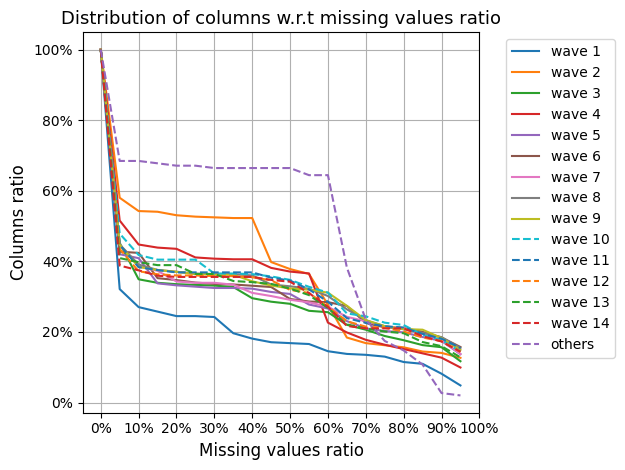
\includegraphics[scale = 0.75]{distribution_of_columns_wrt_missing_values_ratio.png}
	\caption{Distribution of columns with respect to missing values ratio}
	\label{distribution_of_columns_wrt_missing_values_ratio}
\end{figure}
\begin{figure}[!h]
	\centering
	\begin{minipage}{0.45\textwidth}
		\centering
		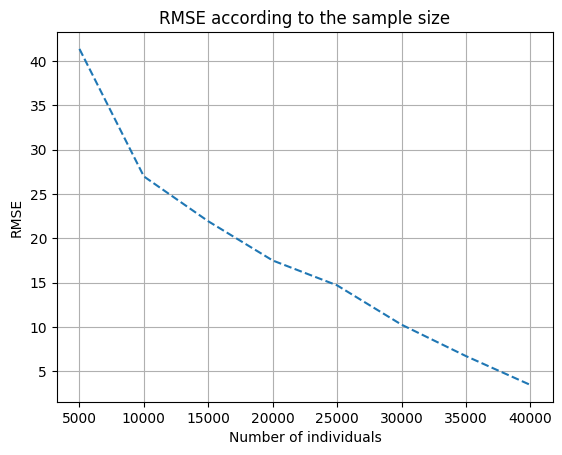
\includegraphics[width=0.9\textwidth]{tSNE_GHI_RMSE_according_to_sample_size.png} % first figure itself
		\caption{RMSE according to the sample size}
		\label{RMSE_according_to_sample_size}
	\end{minipage}\hfill
	\begin{minipage}{0.45\textwidth}
		\centering
		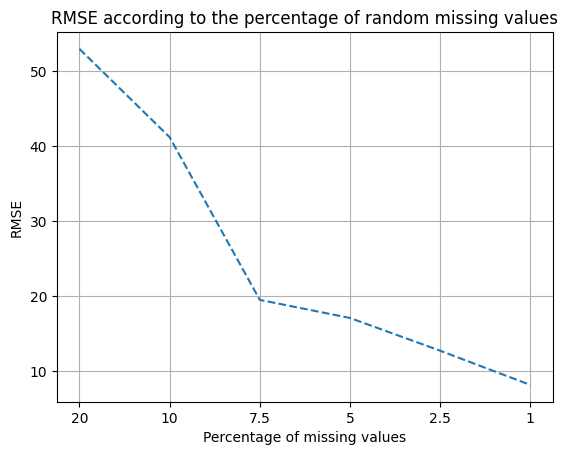
\includegraphics[width=0.9\textwidth]{tSNE_GHI_RMSE_according_to_percentage_NaN.png} % second figure itself
		\caption{RMSE according to NaN percentage}
		\label{RMSE_according_to_percentage_nan}
	\end{minipage}
\end{figure}
\begin{figure}[!h]
\centering
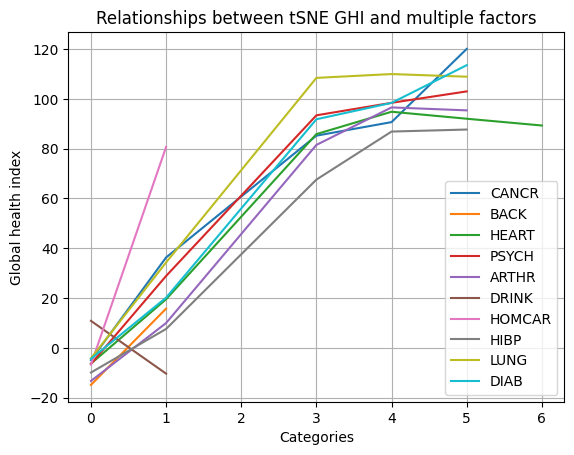
\includegraphics[scale=0.75]{relationships_between_tSNE_GHI_and_multiple_factors.png}
\caption{Relationships between the global health index and multiple factors}
\label{relationships_between_tSNE_GHI_and_multiple_factors}
\end{figure}
\begin{figure}[!h]
\centering
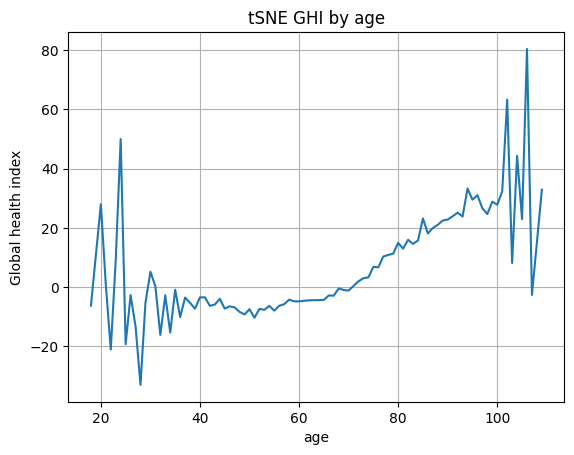
\includegraphics[scale=0.75]{tSNE_GHI_by_age.png}
\caption{Relationship between the global health index and age}
\label{tSNE_GHI_by_age}
\end{figure}
\begin{figure}[!h]
\centering
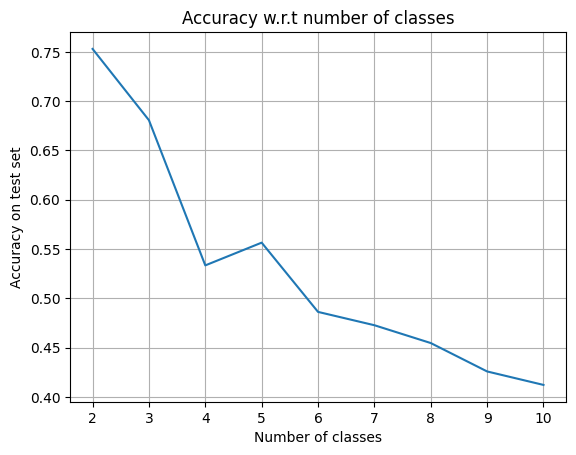
\includegraphics[scale=0.75]{xgboost_accuracy_wrt_number_of_classes.png}
\caption{Accuracy of XGBoost classifier with respect to the number of classes}
\label{xgboost_accuracy}
\end{figure}
\begin{figure}[!h]
	\centering
	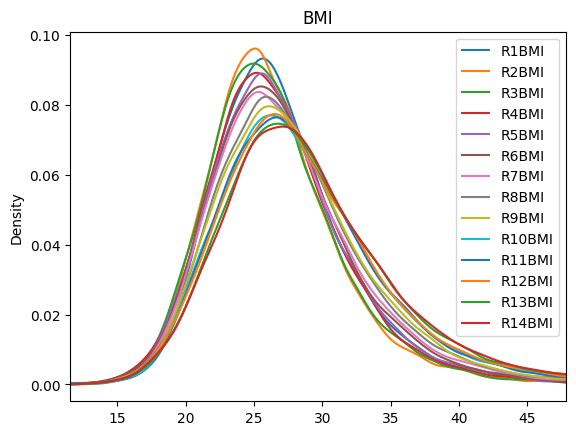
\includegraphics[scale = 0.75]{density_bmi.png}
	\caption{Density of the variable BMI for each wave}
	\label{density_bmi}
\end{figure}
\begin{figure}[!h]
	\centering
	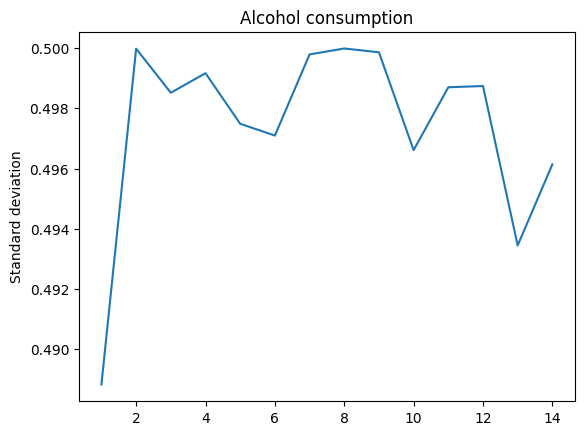
\includegraphics[scale = 0.75]{std_alcohol.png}
	\caption{Standard deviation of the variable measuring alcohol consumption across waves}
	\label{std_alcohol}
\end{figure}
\noindent
Figure \ref{distribution_of_columns_wrt_missing_values_ratio} is meant to be interpreted like this: among the variables collected from the interviews in wave 2, $40$\% of them present more than $45$\% missing values.\\

\noindent
Figure \ref{RMSE_according_to_sample_size} plots the root mean-squared-error observed between the actual index and the index determined on a sample of the data, size of which being informed on the $x$ axis. Figure \ref{RMSE_according_to_percentage_nan} gives the same information for each missing values rate.\\

\noindent
Figure \ref{relationships_between_tSNE_GHI_and_multiple_factors} describes how the GHI is changed when a certain factor is present. The category $0$ stands for \textit{no such factor}, category $1$ for \textit{there is this factor}, and other categories express a higher level of the current factor. For instance, \pyth!DIAB = 0! means that the individual does not present diabete. \pyth!CANCR, BACK, HEART, LUNG! stand for the presence of cancer, of pain or health problems in the back, the heart, or the lung. Overall, what we see was expected: when some one has arthrose problems (\pyth!ARTHR!), his general health is expected to be lower, hence his GHI to be higher. The unique variable that behave differently is \pyth!DRINK!, that describes how much one drinks alcohol. But the deviation is marginal.\\

\noindent
Figure \ref{tSNE_GHI_by_age} highlights the expected fact that someone's health is better when he is young.\\

\noindent
Figure \ref{xgboost_accuracy} gives, for a specific number of classes $c$, the accuracy of the XGBoost classifier, that is the number of correct guesses divided by the number of guesses.

\cleardoublepage
\bibliographystyle{plain}
\bibliography{refs}

\end{document}
